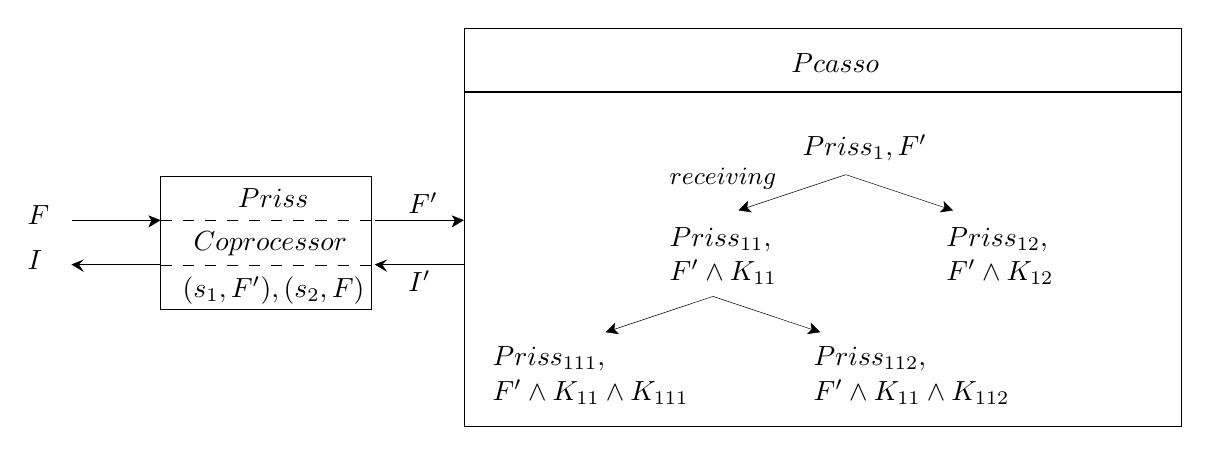
\begin{tikzpicture}[y=0.80pt, x=0.80pt, yscale=-1.000000, xscale=1.000000, inner sep=0pt, outer sep=0pt]

  \path[draw=black,line width=0.160pt,rounded corners=0.0000cm] (370,-453) rectangle (465,-393);
  \path[draw=black,dash pattern=on 4.00pt,line width=0.160pt]   (370,-433)  -- (465,-433);
  \path[draw=black,dash pattern=on 4.00pt,line width=0.160pt]   (370,-413)  -- (465,-413);
  \path[fill=black] (405,-439) node[above right] (text4428) {$Priss$};
  \path[fill=black] (385,-417) node[above right] (text4432) {$Coprocessor$};
  \path[fill=black] (380,-395) node[above right] (text4446) {$(s_1, F'), (s_2, F)$};

  % output arrow
  \begin{scope}[shift={(-130,6.89156)}]
    \path[draw=black,line width=0.160pt] (463,-420) -- (500,-420);
    \path[fill=black] (465,-417) -- (460,-420) -- (465,-422) -- (463,-420) -- cycle;
    \path[draw=black,line width=0.160pt] (465,-417) -- (460,-420) -- (465,-422) -- (463,-420) -- cycle;
  \end{scope}

  % input arrow
  \begin{scope}[shift={(-10,6.89156)}]
    \path[draw=black,line width=0.160pt] (340,-440) -- (376.0260,-440);
    \path[fill=black] (374.7760,-442) -- (379.7760,-440) -- (374.7760,-437) -- (376.0260,-440) -- cycle;
    \path[draw=black,line width=0.160pt] (374.7760,-442) -- (379.7760,-440) -- (374.7760,-437) -- (376.0260,-440) -- cycle;
  \end{scope}

  \path[fill=black] (310,-431) node[above right] (text4466) {$F$};
  \path[fill=black] (310,-411) node[above right] (text4470) {$I$};

  % intermidiate output arrow
  \begin{scope}[shift={(7,6.89156)}]
    \path[draw=black,line width=0.160pt] (463,-420) -- (500,-420);
    \path[fill=black] (465,-417) -- (460,-420) -- (465,-422) -- (463,-420) -- cycle;
    \path[draw=black,line width=0.160pt] (465,-417) -- (460,-420) -- (465,-422) -- (463,-420) -- cycle;
  \end{scope}

  % intermidiate input arrow
  \begin{scope}[shift={(7,6.89156)}]
    \path[draw=black,line width=0.160pt] (460,-440) -- (496.0260,-440);
    \path[fill=black] (494.7760,-442) -- (499.7760,-440) -- (494.7760,-437) -- (496.0260,-440) -- cycle;
    \path[draw=black,line width=0.160pt] (494.7760,-442) -- (499.7760,-440) -- (494.7760,-437) -- (496.0260,-440) -- cycle;
  \end{scope}

  \path[fill=black] (482,-436) node[above right] (text4502) {$F'$};
  \path[fill=black] (482,-401) node[above right] (text4506) {$I'$};

  \path[draw=black,line width=0.160pt,rounded corners=0cm] (507,-520) rectangle (831,-340);

  \path[fill=black] (655,-500) node[above right] (text4498) {$Pcasso$};
  \path[draw=black,line join=miter,line cap=butt,miter limit=4.00,line width=0.435pt] (507,-491) -- (831,-491);

  % level one
  \path[fill=black] (660,-460) node[above right] (text4510) {$Priss_1,  F'$};

  \path[fill=black] (600,-447) node[above right] (text4511) {\small$receiving$};

  % level two
  \begin{scope}[cm={{0.94861,-0.31644,0.31644,0.94861,(255.76474,179.04113)}}]
    \path[draw=black,line width=0.183pt] (555.1339,-466.1446) -- (602.1395,-466.1446);
    \path[shift={(91.12944,-46.14463)},fill=black] (465.2240,-417.5000) -- (460.2240,-420.0000) -- (465.2240,-422.5000) -- (463.9740,-420.0000) -- cycle;
    \path[shift={(91.12944,-46.14463)},draw=black,line width=0.160pt] (465.2240,-417.5000) -- (460.2240,-420.0000) -- (465.2240,-422.5000) -- (463.9740,-420.0000) -- cycle;
  \end{scope}

  \begin{scope}[cm={{-0.94861,-0.31644,-0.31644,0.94861,(1103.2911,179.04114)}}]
    \path[draw=black,line width=0.183pt] (555.1339,-466.1446) -- (602.1395,-466.1446);
    \path[shift={(91.12944,-46.14463)},fill=black] (465.2240,-422.5000) -- (463.9740,-420.0000) -- (465.2240,-417.5000) -- (460.2240,-420.0000) -- cycle;
    \path[shift={(91.12944,-46.14463)},draw=black,line width=0.160pt] (465.2240,-422.5000) -- (463.9740,-420.0000) -- (465.2240,-417.5000) -- (460.2240,-420.0000) -- cycle;
  \end{scope}

  \path[fill=black] (600,-419) node[above right] (text4518) {$Priss_{11},$};
  \path[fill=black] (600,-404) node[above right] (text4519) {$F' \land K_{11}$};
  
  \path[fill=black] (725,-419) node[above right] (text4522) {$Priss_{12},$};
  \path[fill=black] (725,-404) node[above right] (text4523) {$F' \land K_{12}$};


  % level three

  \begin{scope}[shift={(-60,55)},cm={{0.94861,-0.31644,0.31644,0.94861,(255.76474,179.04113)}}]
    \path[draw=black,line width=0.183pt] (555.1339,-466.1446) -- (602.1395,-466.1446);
    \path[shift={(91.12944,-46.14463)},fill=black] (465.2240,-417.5000) -- (460.2240,-420.0000) -- (465.2240,-422.5000) -- (463.9740,-420.0000) -- cycle;
    \path[shift={(91.12944,-46.14463)},draw=black,line width=0.160pt] (465.2240,-417.5000) -- (460.2240,-420.0000) -- (465.2240,-422.5000) -- (463.9740,-420.0000) -- cycle;
  \end{scope}

  \begin{scope}[shift={(-60,55)},cm={{-0.94861,-0.31644,-0.31644,0.94861,(1103.2911,179.04114)}}]
    \path[draw=black,line width=0.183pt] (555.1339,-466.1446) -- (602.1395,-466.1446);
    \path[shift={(91.12944,-46.14463)},fill=black] (465.2240,-422.5000) -- (463.9740,-420.0000) -- (465.2240,-417.5000) -- (460.2240,-420.0000) -- cycle;
    \path[shift={(91.12944,-46.14463)},draw=black,line width=0.160pt] (465.2240,-422.5000) -- (463.9740,-420.0000) -- (465.2240,-417.5000) -- (460.2240,-420.0000) -- cycle;
  \end{scope}

  \path[fill=black] (520,-365) node[above right] (text4530) {$Priss_{111},$};
  \path[fill=black] (520,-350) node[above right] (text4531) {$F' \land K_{11} \land K_{111}$};
  \path[fill=black] (665,-365) node[above right] (text4534) {$Priss_{112},$};
  \path[fill=black] (665,-350) node[above right] (text4535) {$F' \land K_{11} \land K_{112}$};

\end{tikzpicture}
